\chapter{Basics of Cavitation}
\label{chap:chapter1}
\section{Definition of cavitation}

Cavitation occurs when the pressure is lower than the vapor pressure
in a liquid medium at a given temperature. The formation of vapor
bubbles is considered to be void space, a cavity, and a region of the
fluid in which vapor exists are called cavities. These vapor cavities
inside a homogenous liquid (in the absence of bubbles in the fluid
stream) can occur in many different conditions based on the
characteristics of liquids that vary depending on the flow
configuration and the physical properties of the liquid.\\

According to Fran and Michel \cite{FundamentalsofCavitation.2004}
"Cavitation can be defined as the breakdown of a liquid medium under
very low pressure".  This makes cavitation relevant to the field of
continuum mechanics and it applies to cases in which the liquid is
either statics or motion.\\

\section{Tension in Liquid}
Liquid tension is defined as the decrease of pressure P occurring at a constant temperature, 
which might be the pressure P below the saturation vapor pressure $P_v$. Basically, 
the magnitude at which the rupture occurs is the tensile strength of the liquid, represented 
by $\Delta P_C$, and the value of $({P_v}-P)$ is the tension in the fluid, represented as 
$\Delta$P. Often, cavitation refers to the rupture of a liquid at a roughly constant 
temperature. The maximum negative pressure at which water gets ruptured (in the absence of dissolved gas) varies between $-3\cdot 10^9$ to $ -3\cdot
10^{10} $ kg/m$s^2$.
\section{Concept of Vapor Pressure} 
The concept of vapor pressure from the classical thermodynamic
viewpoint in the phase diagram of water is shown in (Figure 1.1). Figure (1.1) shows 
 that the curve from the triple point Tr to critical point C
separates the liquid and vapor domains. The condition of evaporation
or condensation of the fluid at a pressure Pv is known as vapor
pressure and this is the function of temperature T.  Cavitation in
the liquid occurs by lowering the pressure at a constant temperature
as often happens in real fluids. Thus cavitation appears similar to
boiling, with exception of the fact that the driving mechanism is not
the temperature but the pressure change. So the path in the phase diagram
is said to be isothermal.\\


\begin{figure}[H]
    \centering
    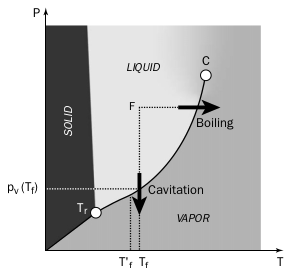
\includegraphics[scale=0.4]{phase diagram.png}
    \caption{phase diagram\cite{FundamentalsofCavitation.2004}}
    \label{fig:fig1}
\end{figure}

 
Several steps can be distinguished during the first instants of
cavitation:

\begin{itemize}
  \item breakdown or void creation,
  \item filling of this void with vapor,
  \item eventual saturation with vapor.
\end {itemize}

In reality, the phases are simultaneous with the second step, so
instantaneous saturation of the void with vapor can be justifiably
assumed. It should be kept in mind that from the phase diagram the
curve Pv(T) is not an absolute boundary between liquid and vapor
states. Deviation from this curve can also make the water not change
its phase, even if a drop in pressure well below the vapor pressure
occurs. This was explained by Andrews-isotherms (Figure 1.2) in the
p-v diagram; the curves can be approximated in the liquid and vapor
domains by the van der Waals equation of state. The transformation
from liquid to vapor along the path AM can be avoided, because the
liquid is in metastable equilibrium and it can even withstand negative
absolute pressure i.e, tension, without any phase change. When treating water in such cases, special care must be taken.\\

\begin{figure}[H]
    \centering
    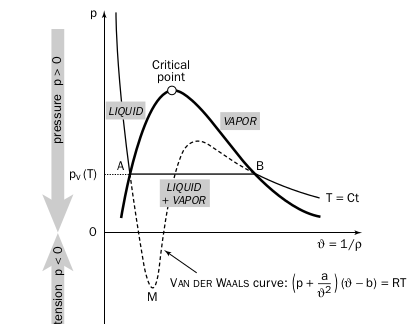
\includegraphics[scale=0.4]{ANDREW ISOTHERM.png}
    \caption{Andrews-isotherms\cite{FundamentalsofCavitation.2004}}
    \label{fig:fig2}
\end{figure}

In summary, Cavitation may or may not occur regardless of whether the
local absolute pressure is equal to or less than the vapor pressure at 
the given global system temperature. The reason for this is because 
fluids have a metastable equilibrium. This difference between the vapor pressure and
absolute local pressure at cavitation inception (the first point about
which phase changes start to generate vapor bubbles) is called static
delay. In some cases, there is also dynamic delay is associated with
inertial phenomena with the time necessary for vapor cavities to be
observable.\\

\section{The Main Forms of Vapor Cavities}
Cavitation patterns of vapor structures can be divided into three
forms. These are:

\begin{itemize}
\item Transient isolated bubbles: These appear in the region of low
  pressure well below the vapor pressure as a result of the rapid
  growth of very small air nuclei present in the liquid. They are
  carried along the stream and modify the flow. As they enter into a
  region of high pressure they progressively disappear.
\item Attached or Sheet Cavities: Such cavities are often attached to
  the leading edge of the body.
\item Cavitating Vortices: Cavitation can appear in the low-pressure
  core of the vortices in the turbulent wake.
\end{itemize}

Some vapor structures with a short lifetime that appear on the surface
of the foils or propeller blades do not fall under these three forms;
even though they have the form of attached cavities, they are
transported similarly to traveling bubbles. This type of form is relevant for the present work.\\

\section{Cavitation Regimes}
For practical purposes, it is necessary to classify the cavitation
region.

\begin{itemize}
\item Cavitation Inception: The limiting regime between the
  non-cavitating condition and the cavitating flow.
\item Developed Cavitation: There is an extent of the
  cavitation zone or significant fall in the performance of the
  machines.
\end{itemize}

In the present work, we are mainly concerned about the extended region of the
cavitation zone where there will be a high influence on unsteady
cavitation shedding. The influencing situation that is favorable for
the cavitation is wall geometry that gives rise to the local
increment in the velocity with the drop in local pressure, and shear
flows due to large turbulent pressure fluctuations.\\

\section{Introduction to Nucleation}
Small gas or vapor inclusions present in a liquid medium act as points of weakness. 
These are known as cavitation nuclei. During the experiment, this point of weakness 
acts as a starting point for the liquid to begin to break down, and it is a few micrometers 
to several hundred micrometers in diameter. They remain spherical at this scale due to 
surface tension. There are two types of nucleation:

\begin{itemize}
\item Homogeneous nucleation: When the pressure is well below the
  saturation pressure the liquid form temporary, microscopic voids
  that can constitute the nuclei, necessary for rupture and growth of
  bubbles.
\item Heterogeneous nucleation: Nucleation can happen at the liquid-solid boundary, 
or as a result of contaminant very small sub-micron sized particles in the liquid, 
or as a result of contaminant gas particles as micro-sized bubbles that can be 
found in crevices within the solid boundary, within suspended particles, 
or freely suspended in the liquid, causing weakness in the fluid under operation. 
\end{itemize}

Kinetic theories have also been developed to cover such heterogeneous
nucleation and allow us to evaluate whether the chance that this will
occur is larger or smaller than the chance of homogeneous nucleation.
Another effect is called cosmic radiation which has less impact on contributing nucleation in a fluid medium. The cosmic
radiation i.e. the collision of molecules due to high energy photon
cause nucleation, but it has little chance to occur so we neglect
these effects. In most cases, heterogeneities inside
the homogeneous medium is taken into consideration because it is
inevitable.\\ One must not forget that it is impossible to completely remove  contaminated gas from water, 
so this effect must be taken into account. Numerical simulations cannot include this point 
of weakness, so external parameters have to be implemented to mimic these effects. 
It is for this reason that cavitation number and cavitation inception have been introduced 
in this work. These non-dimensional numbers can be extracted through experiments.\\

\section{Homogeneous Nucleation Theory}
This theory is the basic understanding
of the Rayleigh-Plesset equation which is a basic traveling bubble
transport equation that will be explained further.\\ Consider a
spherical microbubble, containing gas and vapor (heterogeneous nuclei
over homogeneous nuclei) in equilibrium within the liquid at
rest. The liquid can withstand negative pressure which means that
is in a metastable state according to the Andrews-isotherm curve (Figure
1.2). The bubble radius R is sufficiently small so that the
hydrostatic pressure $2\rho gR$ can be neglected in comparison with
surface tension 2S/R. This condition requires R to be smaller than
the limiting value namely 2.7mm for water. To 
fulfill this condition the microbubble whose diameter is
smaller than 0.5mm only are considered. The pressure can be uniform
in the bulk of the surrounding fluid where there is the bubble and
this microbubble is spherical. The spherical shape in the bubble is
mainly due to the surface tension which states that "intermolecular
forces that tend to hold the molecules together and prevent the
formation of the large hole".\\

\begin{figure}[H]
    \centering
    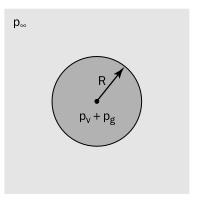
\includegraphics[scale=0.5]{bubble force equilibrium.png}
    \caption{Microbubble in liquid \cite{FundamentalsofCavitation.2004}}
    \label{fig:fig3}
\end{figure}

The pressure equilibrium of the interface between the fluid
surrounding and bubble surface is given by:\\
\begin{equation}
P_{\infty} =P_g + P_v -\frac{2S}{R}
\end{equation}

${P_\infty}$ is the surrounding bulk uniform pressure,$P_g$ gas
pressure inside the bubble,$P_v$vapor pressure,S surface tension,R
radius of the bubble.\\ It is assumed that pressure change is slow
enough to achieve mechanical equilibrium. However, the change in
pressure must be rapid enough to ensure the gas diffusion at the
interface is negligible.  In other words, the transformation is
assumed to be isothermal and the mass of the gas inside the bubble is
constant.\\ For the initial state,denoted by subscript 0,
equation(1.1) is written as follows:
\begin{equation}
P_{{\infty}{0}} =P_{g0}+P_v-\frac{2S}{R_0}
\end{equation}

As the gas pressure is inversely proportional to the volume in the
isothermal transformation, then from equation (1.1) one can obtain:
\begin{equation}
P_{\infty} =\frac{P_{g0}}{{[{R_0}/{R}]}^{3}} +P_v -\frac{2S}{R}
\end{equation}

assuming that the critical nucleus is in thermodynamic equilibrium
with its surrounding after its creation. The critical radius and
critical pressure are given by comparing equation (1.1) and (1.2) by
assuming virtual transformation from initial radius to critical radius
under the isothermal condition with the mass of gas. Two mechanisms
take place in equation (1.1), they are:

\begin{itemize}
  \item the internal pressure effect which tend to increase the bubble
    size,to reach critical size.
  \item the surface tension effect which act in the opposite direction
    resulting in  minimum extension are given by:
\end{itemize}

\begin{equation}
R_C = R_0 \frac {3P_{g0}}{[{\frac{2S}{R_0}}]^{1/2}}
\end{equation}
  
\begin{equation}
  P_C = P_v -{\frac{4S}{3R_C}}
\end{equation}

The mass of gas inside the bubble is said to be constant and it is directly proportional
to the $P_{g0}{{R_0}^3}$. To use the condition of a constant mass of
gas either use one of the doublets ($R_0 ,P_{\infty}$), ($R_0,P_{g0}$)
or preferably one of the quantities $R_c$ or $P_c $. The stability of the
nucleus is given in (Figure 1.4) in which the mechanical equilibrium of
the specific nucleus is stable on the branch of the curve that has a
negative slope. The other branch which is on the right side is said to
be unstable.\\

\begin{figure}[H]
  \centering
  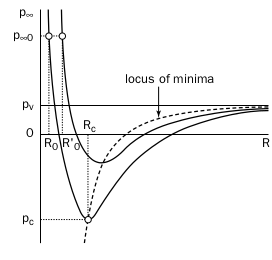
\includegraphics[scale=0.5]{stability curve.png}
  \caption{Equilibrium of a sphere nucleus \cite{FundamentalsofCavitation.2004}}
  \label{fig:fig4}
\end{figure}

\section{Concept of Cavitation Number}
The coefficient of pressure $C_{pmin}$ for an ideal fluid is dependent
on geometry when the effect of viscosity is included the $C_{pmin}$ is
also a function of Reynolds number $R_e$. For this instance just
consider  the $C_{pmin}$ as a function of geometry only, which is stated in \cite{CavitationandBubbleDynamics.1995}.
    
\begin{equation}
C_{px} =\frac {P_x-P_{\infty}}{{0.5 \rho {U^{2}_{\infty}}}}
\end{equation}

Cavitation occurs when the pressure is less than saturation pressure at a given temperature.
This natural event can be formulated through a non-dimensional term called cavitation number $\sigma$. The cavitation
number $\sigma$ are related with the $C_{pmin}$ thanks to the following.
\begin{equation}
\sigma =\frac{{P_{\infty}}-{{P_v}(T_{\infty})}}{{0.5 \rho {U^{2}_{\infty}}}}
\end{equation}

The nucleation that will initially encounter at some point in the flow field is called cavitation 
inception for a sufficiently small value of $\sigma$ (which means $P_{\infty}$  is sufficiently 
smaller than $P_v$ and $U_{\infty}$ is sufficiently greater).
The cavitation inception, also known as the lowest pressure point around which nucleation begins to form, appears to be observable.
There is an increase in the formation of bubbles in the flow as $\sigma$ is reduced more below $\sigma _{i}$. 

\begin{equation}
{{\sigma}_i} =-C_{pmin}
\end{equation}

From Figure (1.5), for $\sigma >$ $-C_{pmin}$ the pressure along the
entire trajectory is greater than vapor pressure $P_v$ and still
non-cavitating condition is respected. For $\sigma =$ $-C_{pmin}$,the
nucleus encounters $P=P_v$ only for an infinitesimal moment. Thus the observation of nuclei is limited or might not be observed. For $\sigma
<$ $C_{pmin}$, the nucleus experience $P<P_v$for a finite time. Thus  
it is observable and they travel along the streamline.\\


\begin{figure}[H]
    \centering
    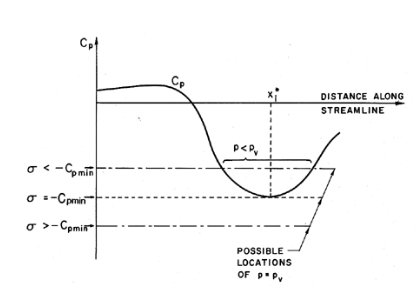
\includegraphics[scale=0.5]{pressure distribution for cp.png}
    \caption{Schematic of pressure distribution on a streamline\cite{FundamentalsofCavitation.2004}}
    \label{fig:fig5}
\end{figure}
So far as free stream nuclei (heterogeneous nuclei) are concerned
two main factors that cause ${\sigma}_i$ be different from $C_{pmin}$.
The first nucleation may not occur at $P=P_v$. In a degassed liquid,
nucleation requires positive tension $\Delta P_c$ and hence nucleation
would require the cavitation number ${{\sigma}_i} <$$C_{Pmin}$, namely
the equation relating the terms like $C_{pmin}$ and tension of the
fluid i.e.  ${{\sigma}_i}=$${-C_{pmin}}-$$\frac {{\Delta}P_c}{0.5 \rho
  {{{U}^2}_\infty}}$. In a liquid containing great deal of contaminant
gas $\Delta P_c$ could be negative so that ${\sigma}$ would be larger
than ${-C_{pmin}}$under the condition $P<{P_v}-$${\Delta}P_c$. This
makes the ${{\sigma}_i}<$${-C_{pmin}}-$$\frac {{\Delta}P_c}{0.5 \rho
  {{{U}^2}_\infty}}$. All these conditions should respect the
assumption of isothermal. If we include the temperature then
${\sigma}_i$will also be a function of Temperature. When there is a great deal of contaminant gas the
tension of the fluid ${\Delta}P_c$ is negative. This means less
tension and a rupture of fluid that occurs faster as the fluid tend to avoid the metastable
equilibrium. In another sense, positive tension in the case of
degassed fluid provides control in cavitation. So not only the
geometry but also treating fluid for the experiment is also
contributing to the cavitation.

\section{Viscous effect in cavitation inception}
In real fluid, $C_{pmin}$ is
not only the function of geometry but also the contribution by the
viscosity. To include this effect of viscosity the $C_{pmin}$ would be
a function of Reynolds number,$R_e$ so the cavitation
inception,${\sigma}_i$ is a dependence of Reynolds number $R_e$. In
most engineering applications the flow is said to be turbulent so
the vortices occur not only because of the inheritance of turbulence
but also due to the free and forced shedding of vortices. This has major
consequences in the cavitation inception ${\sigma}_i$ because the
pressure at the center part of the vortices is lower than the mean
pressure in the flow. For this reason, the cavitation first occurs at the core and
${\sigma}_i$  changes with $R_e$. There are a few other effects that make the
${\sigma}_i$ to be more complicated in measurement through experiment:


\begin{itemize}
  \item Existence of tensile strength can cause a reduction in
    ${\sigma}_i$.
  \item Residence time effects can cause a reduction in ${\sigma}_i$.
  \item Existence of contaminated gas can cause an increase in
    ${\sigma}_i$.
  \item Steady viscous effect due to dependence of $C_{pmin}$ on $R_e$
    can cause ${\sigma}_i$ to be function of $R_e$.
  \item Turbulence effect can cause an increase in ${\sigma}_i$
\end{itemize}

If  these  effects are not included then ${\sigma}_i$ is the only function
of $C_{pmin}$. Some of the experimental techniques which are used to
measure the ${\sigma}_i$ are based on acoustic scattering
and light scattering. These have been used to measure the number of nuclei
present in the liquid. Other instruments known as cavitation
susceptibility meters cause a sample of liquid to cavitate and measure
the number and size of the resulting microscopic bubbles. The
discussion of this technique is out of the scope for this document.


\section{Types of Cavitation}

\subsection{Travelling Bubble Cavitation}
The bubble began as micron-sized nuclei in the liquid of the oncoming
stream and the bubble moved with the flow free stream velocity close
to the solid body.Cavitation inception was deemed to occur when the
bubble reaches an observable size.

\begin{figure}[H]
  \centering
  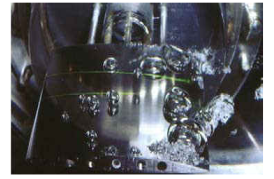
\includegraphics[scale=0.6]{travellingbubble.png}
  \caption{Travelling bubble on the surface of an hydrofoil \cite{FundamentalsofCavitation.2004}}
  \label{fig:fig6}
\end{figure}

\subsection{Vortex Cavitation}
This type of cavitation comes under large-scale cavitation
structures. Cavitation inception often occurs at the core of the
vortices when the core pressure is well below the mean flow pressure.
For high $R_e$ the vortices in a turbulent mixing layer or wake will
also cavitate. This type is often seen in the tip vortices in the
ship's propellers or pump impellers.  The three-dimensional shedding
of vortices from a finite aspect ratio foil often leads to the
formation and propagation of a ring vortex with a vapor core.

\begin{figure}[H]
 \centering
 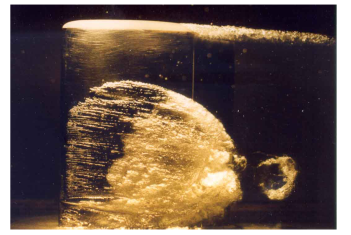
\includegraphics[scale=0.5]{Vortexcavitation.png}
 \caption{ring vortex on the surface of an hydrofoil \cite{FundamentalsofCavitation.2004}}
  \label{fig:fig7}
\end{figure}
\subsection{Cloud Cavitation}

This is another class of large-scale cavitation. The periodic
formation and collapse of a cloud of cavitation bubbles are
observed. This topic is more pertinent to the current project.

\begin{figure}[H]
 \centering
 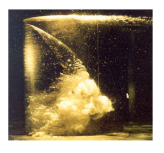
\includegraphics[scale=1]{cloudshedding.png}
 \caption{Cavitating cloud on hydrofoil \cite{FundamentalsofCavitation.2004}}
 \label{fig:fig8}
\end{figure} 

\subsection{Shear Cavitation}
The region with high shear vorticity produces.  As a result, a
coherent rotational structure is formed and pressure levels drop in
the core of the vortices which became the potential site for the
cavitation. This often happen in the flow separation region which is
developed by the hydrofoil at very high $R_e$ and angle of attack.

\begin{figure}[H]
 \centering
 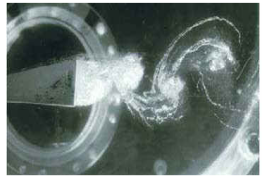
\includegraphics[scale=0.6]{shearcavitation.png}
 \caption{Shear Cavitation \cite{FundamentalsofCavitation.2004}}
  \label{fig:fig9}
\end{figure}

\subsection{Attached/Sheet Cavitation}
These types of cavitation are often experienced in hydrofoils. The present
work focused on simulation of Attached/Sheetcavitation along with closed type partial cavitation through the case
setup and this is the area of interest to replicate the unsteady
behavior of cloud shedding.\\

\textbf{SuperCavitation}: As the cavitation parameter is decreased a
small cavity attached to a hydrofoil will extend to grow longer and
longer as can see in figure (1.10). The super cavity as soon as it ceases to close the
cavitation wall but inside the liquid downstream of the
cavitation. As a consequence, the lift of the foil will decrease with an increase in
drag. For lower cavitation numbers which mean low $R_e$
the supercavitation is experienced in the foil and cavity closure
occurs at the rear part. Because of the low Reynolds number $R_e$ laminar
separation boundary layer will experience over the hydrofoil as the angle of attack increases. 
A well-developed cavity always detached downstream of
the laminar separation of the boundary layer. The existence of separation,
which generates a relatively dead zone near the downstream is the only
way for the cavity to get attached to the wall i.e, turbulent reattachment. 
On the other hand, if there is no reattachment then the cavity will sweep away by the flow.  
In addition to turbulent reattachment, there is a  cavity closure region near the downstream
 because the pressure inside the cavitation zone is less than surrounding freestream pressure. 
The unbalance inertia and pressure force gives a
curvature oriented toward the cavity.\\

\begin{figure}[H]
 \centering
 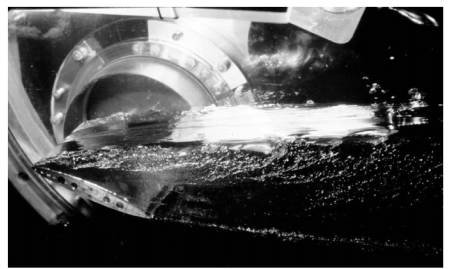
\includegraphics[scale=0.4]{supercavitation.png}
 \caption{Supercavity behind two dimensional hydrofoil \cite{FundamentalsofCavitation.2004}}
  \label{fig:fig10}
\end{figure}

\textbf{Partial Cavitation}: In partial
cavitation, the attached cavity closes on the suction side of the
hydrofoil. This type of cavitation has two types:

\textbf{Open attached cavity -partial type}:   From the reference \cite{ceccio2001}, 
the authors investigate the NACA0009 hydrofoil under cavitation conditions. 
They concluded that an open attached partial type cavity is typically frothy in
appearance and has periodically varying lengths, which is associated
with the shedding of vapor clouds. Although recirculation flow related to the region 
of flow separation, i.e. turbulent reattachment, was recorded in the cavity closure, the re-entrant jet was not observed.
The re-entrant jet in an open cavity is not observed due to conditions linked to the 
maximum cavity thickness, which is not reached in the open cavity. This is because there exists 
a low cavitation number associated with low angles of
attack in the case of hydrofoils which can be seen in the
figure(1.12).\\ 
\textbf{Closed attached cavity-partial cavity}: From the observation of 
authors \cite{ceccio2001}, they concluded that this type of cavity has a
relatively stable cavity length, a clear interface, and a cavity
the closure that is relatively free from the bubble and  entirely vapors
fill. This demonstrates an important aspect of introducing the single-phase flow
concept by considering the vapor-filled state, because bubble interaction is completely
removed, as stated in the above statement of the closed partial cavity, and assuming
the relative velocity between these two phases is zero, the flow now completely transfers
to a single-phase flow regime. This simulation adapts closed type partial cavitation 
for unsteady cloud shedding and re-entrant jet observation. \\

\begin{figure}[H]
  \centering
  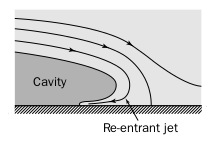
\includegraphics[scale=1]{reentantjet.png}
  \caption{closure region of partial cavity \cite{FundamentalsofCavitation.2004}}
  \label{fig:fig11}
\end{figure}

\textbf{Unsteady Re-entrant jet}: The re-entrant jet proceeds from upstream, carrying a tiny amount of liquid inside 
the cavity, and the outside section is reattached by turbulent reattachment, as shown in figure (1.11). 
If the cavity interface is close to the suction rear side, where maximum cavity length is seen, 
a reentrant jet with an energetic flow will be able to cut the cavity interface when this 
re-entrant jet impinges on the cavity interface. It will induces a periodic break-off 
and roll-up of a part of the cavity. If the
re-entrant jet moves far upstream, it causes a large portion of the
cavity to break off then the process creates large-scale cloud shedding. If
they move to a smaller distance upstream before impingement on the
cavity surface then the process is called small-scale cloud
cavitation.

From the figure(1.12) we can see that the open cavity at low
cavitation and low angle of attack where the re-entrant is not
observed or weak in re-entrant flow but there is a turbulent
reattachment. At the same time in the periodic zone regime, we can see
cloud shedding at a higher angle of attack and higher cavitation
number along with the ratio of cavitation thickness to the chord $e/c$
is minimum and the ratio of the length of the cavity to chord $l/c$ is
around half the length of the chord act as a maximum $l/c$ i.e. a
peculiar instability develops for partial cavities of medium
length. On the other hand, it was limited by the minimum cavity
thickness. Such limits suggest that a minimum value of cavity
thickness is required for the periodic regime to develop. This also
shows that cavity thickness must be larger than the re-entrant jet
thickness for this instability to occur along with another condition
like the periodic regime is bounded by the maximum value of the cavity
length which indicates that instability should not occur for very long
cavities. This condition also holds for the re-entrant jet which
requires a minimum threshold value of the adverse pressure gradient to
gain the impulse. Finally, to generate partial periodic cavity shedding 
and an energetic re-entrant jet, there must be a minimum cavity thickness
to chord ratio and a maximum length of the cavity to chord ratio. \\

\begin{figure}[H]
 \centering
 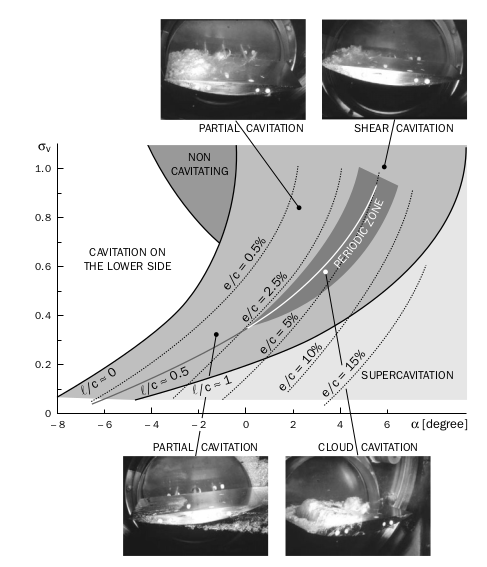
\includegraphics[scale=0.4]{partialcavitation.png}
 \caption{Main cavity patterns at $R_e =$ $2.{10}^6$ ${V_{\infty}}
   =10{m}/{s}$ on plano-circular hydrofoil \cite{FundamentalsofCavitation.2004}}
  \label{fig:fig12}
\end{figure}

\section{Three dimensional effect in hydrofoil}
The transition of sheet cavitation to cloud cavitation can result in a
highly unstable flow. To study cavitation-vortex
interaction\cite{JI2015}, the vorticity transport equation in a
varying density flow is given as
\begin{equation}
\frac{D\omega}{Dt}=({\omega.\triangledown})\vec{V}
-\vec{\omega}(\triangledown.\vec{V}) + \frac{{\triangledown{\rho}_m}
  {\times\triangledown P}}{{{\rho}^2}_m} +({\nu}_m
+{\nu}_t){{\triangledown}^2}\vec{\omega}
\end{equation}

In this equation, the first term on the right-hand side (RHS) is the vortex 
stretching the term. The term describes the stretching and tilting of a vortex 
caused by velocity gradients. On the right, the second term is the vortex dilation 
term due to volumetric expansion or contraction, which describes how fluid 
compressibility affects vorticity. The third term on the RHS is the baroclinic 
torque, which is a result of misaligned pressure and density gradients. 
The last term on the RHS indicates how fast the vorticity changes as a 
result of viscous diffusion. It is significant to realize that the viscous 
diffusion term in high $R_e$ has a much smaller effect on the vorticity transport 
than the other three terms because the inertia force is more dominant away from 
the wall. The numerical and experimental studies show that the shedding vapor has a 
strong vortex-cavitation interaction, with vortex stretching and dilatation 
being the primary mechanism of cloud transition from 2D to the 3D cloud. 
As the shedding vapor cloud collapses downstream, the attached cavity 
shrinks quickly, changing from 3D to 2D.  During this process, the attached sheet
cavity and the boundary layer become very thin. The strength of the
vortex stretching term and dilatation term decreases significantly
with the extent of the cavitation region. Even though the baroclinic
torque term has a smaller magnitude than the vortex stretching and
dilatation terms, it is very important for the production of vorticity
and modifies the vorticity field in regions with high density and 
pressure gradients, such as near the cavity closure and along with
the liquid-vapor interface. Despite the fact that it is an unrelated issue for this project, 
it is critical to comprehend the 3D effect in hydrofoils and 
how this effect is reflected in the results when comparing 
numerical 2D with experimental results. 

\section{Main Effect of Cavitation in Hydraulics Performance}
Several consequences of cavitation can be expected as:
\begin{itemize}
\item Drops in hydraulics system performance, for example, decreases 
in lift and drag increases of the foil, decreases in turbomachinery 
efficiency, lower ability to evacuate water in spillways, energy dissipation, and so on. 
\item It contributes to the production of noise and vibration which damages the structures,
\item Wall erosion when the bubble gets extruded between the fluid and
  solid surface the solid surface is eroded. This effect acts
  like a creep and it reduces the  machine's usable lifetime.
\end{itemize}
